\documentclass[11pt,oneside]{book}

\usepackage[T1]{fontenc}
\usepackage[utf8]{inputenc}
\usepackage[margin=1in]{geometry}
\usepackage{amsmath,amssymb}
\usepackage{graphicx}
\usepackage{array}
\usepackage{booktabs}
\usepackage{longtable}
\usepackage{enumitem}
\usepackage{xcolor}
\usepackage{listings}
\usepackage[obeyspaces]{xurl}
\usepackage[hidelinks]{hyperref}

\graphicspath{{figures/}}

\lstdefinestyle{terminal}{
  basicstyle=\ttfamily\small,
  breaklines=true,
  frame=single,
  columns=fullflexible,
  keepspaces=true,
  showstringspaces=false,
  backgroundcolor=\color{black!3}
}
\lstset{style=terminal}

\newcommand{\semdsm}{SEM--DSM}
\newcommand{\specfem}{SPECFEM3D}
\newcolumntype{L}[1]{>{\raggedright\arraybackslash}p{#1}}
\urlstyle{tt}
\DeclareRobustCommand{\code}[1]{\nolinkurl{#1}}
\newcommand{\dd}{\mathrm{d}}

\title{\textbf{SEM--DSM Hybrid Method Manual}\\
\large A practical guide for localized 3-D teleseismic waveform modelling}
\author{Wenbo Wu}
\date{\today}

\begin{document}
\frontmatter
\maketitle
\tableofcontents

\chapter*{Scope}
\addcontentsline{toc}{chapter}{Scope}

This manual describes the practical workflow for running the \semdsm{}
hybrid method implemented in this repository. The method combines the Direct
Solution Method (DSM), which computes wave propagation in a 1-D spherical
Earth model, with a localized 3-D \specfem{} simulation. The 1-D incident
wavefield is injected into a small SEM box that contains the target 3-D
heterogeneity, and the scattered wavefield recorded on an internal coupling
boundary is extrapolated to teleseismic receivers with DSM Green's functions.

The manual is written for users who want to run or adapt the example cases.
The main user-facing workflow is controlled by a case directory. Its
\code{DATA/} directory contains the configuration and Fortran model sources,
including \code{model_tomography.f90} and \code{get_model.F90};
\code{auxiliary/} contains the helper programs; and the \code{step*.sh}
scripts drive the workflow. Each case has a Step~0 script that activates its
SPECFEM3D database-model sources before the remaining workflow is run.

\mainmatter

\chapter{Introduction}

\section{Why a hybrid method}

Fully global 3-D simulations at frequencies near 1 Hz are usually too
expensive for routine teleseismic modelling. In many applications the
structure of interest is localized: an ultra-low velocity zone near the CMB,
topography on the ICB, or small-scale inner-core heterogeneity along one
ray bundle. The \semdsm{} method exploits this localization. The global
background propagation is handled by DSM in a 1-D Earth model, while the
expensive 3-D calculation is restricted to a small box around the target
region.

\begin{figure}[htbp]
  \centering
  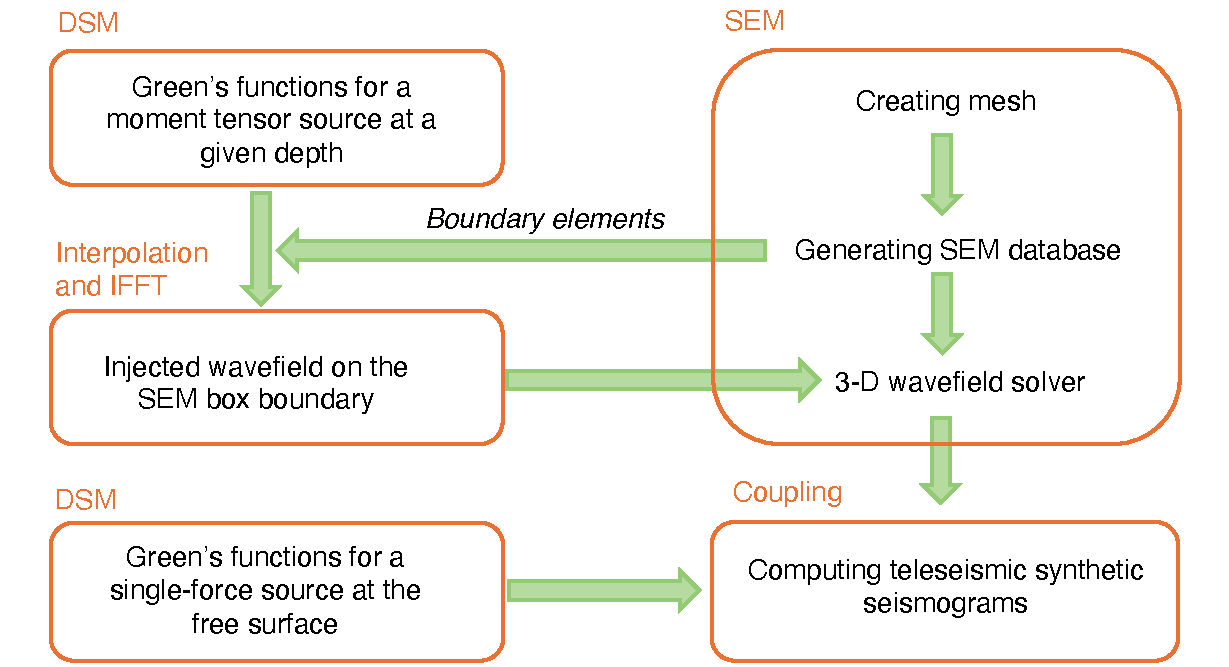
\includegraphics[width=0.88\textwidth]{workflow_ReducedSize.pdf}
  \caption{High-level workflow of the \semdsm{} hybrid method. DSM is used
  for source-to-box, box-to-receiver, and reference 1-D synthetics. The
  source-to-box DSM wavefield is converted to the injected wavefield used by
  \specfem{}. The \specfem{} boundary displacement and traction are combined
  with box-to-receiver DSM Green's functions to produce scattered teleseismic
  synthetics.}
  \label{fig:workflow}
\end{figure}

\section{Coupling concept}

Let the Earth be divided into an exterior domain \(V_1\), which contains the
earthquake source and teleseismic receivers, and a localized 3-D SEM domain
\(V_2\), which contains the target structure. The interface used for
reconstructing the scattered wavefield is \(S_{12}\). In the exterior
domain the wavefield is represented by 1-D DSM Green's functions:
\begin{equation}
\begin{aligned}
u_n^{\mathrm{scat}}(\mathbf{x},t)
=
\int_{-\infty}^{\infty}
\int_{S_{12}}
\left[
G_{ni}^{1D}(\mathbf{x},t-\tau;\boldsymbol{\xi},0)
T_i^{3D}(\boldsymbol{\xi},\tau)
-
u_j^{3D}(\boldsymbol{\xi},\tau)
C_{jklm}^{1D}(\boldsymbol{\xi})
\frac{\partial G_{nm}^{1D}}{\partial \xi_l}
n_k
\right]
\dd S\,\dd \tau .
\end{aligned}
\label{eq:coupling_integral}
\end{equation}
The full teleseismic waveform is the sum of the DSM 1-D reference waveform
and the scattered waveform from Eq.~\ref{eq:coupling_integral}.

\begin{figure}[htbp]
  \centering
  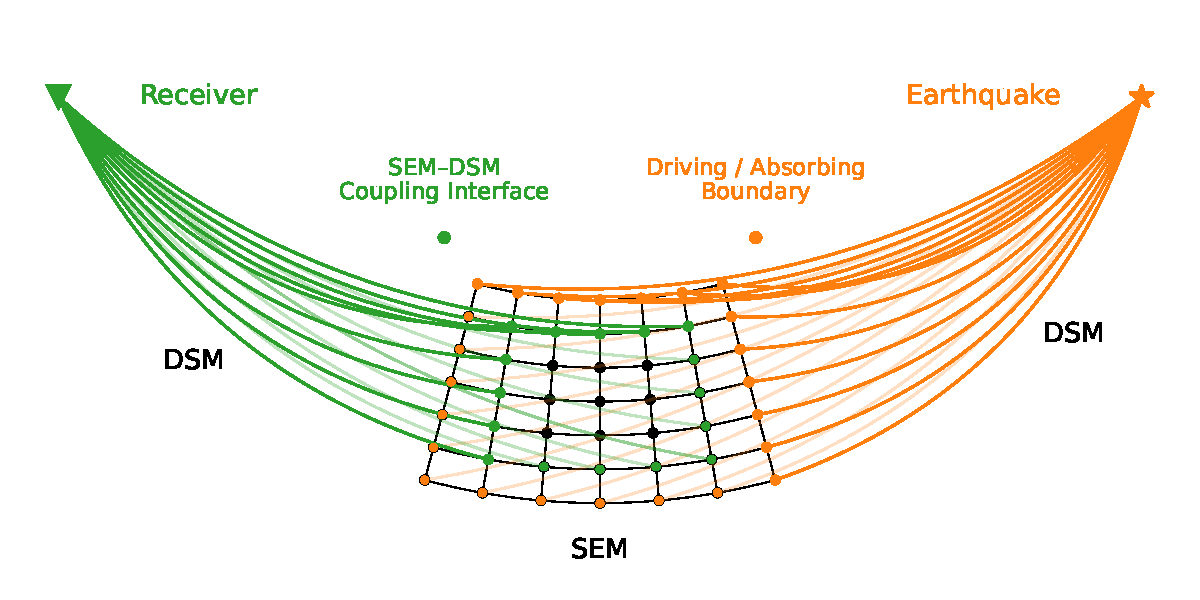
\includegraphics[width=0.72\textwidth]{DSM_SEM.pdf}
  \caption{Schematic \semdsm{} coupling geometry. The outer SEM boundary is
  driven by the injected DSM incident wavefield. The internal coupling
  boundary provides the displacement and traction used in the representation
  theorem. Absorbing boundaries remove outgoing scattered waves.}
  \label{fig:dsm_sem}
\end{figure}

\section{Directory layout}

A typical example directory has the following structure:
\begin{lstlisting}
Example_case/
  DATA/
    Par_file_SEM_DSM
    CMTSOLUTION
    dsm_model_base
    model_tomography.f90
    get_model.F90
    tele_station.txt
  auxiliary/
    select_generate_databases_model.sh
    prepare_src_to_box.py
    prepare_box_to_recv.py
    prepare_injected_waves.py
    assemble_3d_sem_dsm_synthetics.py
  step0_prepare_*.sh
  step1_specfem_mesh_database.sh
  step2_3Dmodel_implementation.sh
  step3_submit_specfem_mesh_gen.sh
  step4_dsm_src_to_box.sh
  step5_dsm_box_to_recv.sh
  step6_1d_dsm_synthetics.sh
  step7_extract_injected_waves.sh
  step8_specfem_solver.sh
  step9_coupling.sh
  step10_assemble_3d_sem_dsm_synthetics.sh
\end{lstlisting}

Each case contains one \code{step0_prepare_*.sh} script. The descriptive
suffix varies with the example because Step~0 may also prepare topography or
volumetric heterogeneity files.

Steps~1--10 write most generated products under \code{WORK/}. Step~0 may
also write case-specific structural inputs under \code{DATA/}. Large completed
products, such as reusable DSM databases or final synthetics, are often saved
as \code{OUTPUT_FILES_*} directories by individual examples.

\chapter{Compile Codes}

\section{Prerequisites}

The code is intended for an MPI-enabled HPC environment. A typical build needs
Fortran, C, MPI compiler wrappers, \code{make}, Python 3, and a Slurm runtime
for the example submission scripts. The standalone component Makefiles use
commands such as \code{gfortran}, \code{gcc}, \code{mpif77}, \code{mpif90},
and \code{mpicc}. For SPECFEM3D, select the serial Fortran, MPI Fortran, and C
compilers with the \code{FC}, \code{MPIFC}, and \code{CC} arguments to
\code{configure}. Edit compiler variables directly only for components that do
not use \code{configure}.

\section{Build order}

From the repository root that contains \code{src/DSM}, \code{src/InjectedWaves},
\code{src/Coupling}, and \code{src/SPECFEM3D}, build the components in this
order:
\begin{lstlisting}
cd src/DSM/src/DSM_Solver
make clean
make

cd ../DSM_FreqToTimeSac
make clean
make

cd ../../../InjectedWaves/src
make clean
make

cd ../../Coupling/src
make clean
make

cd ../../SPECFEM3D
./configure FC=gfortran MPIFC=mpif90 CC=mpicc
make
\end{lstlisting}

The \code{xcubedsphere_topo} program converts geographic interface topography
to the cubed-sphere grid used by topographic SEM meshes. It is compiled with
the other default SPECFEM3D executables when \code{make} is run.

Then change into the selected example directory and run its Step~0 script:
\begin{lstlisting}
./step0_prepare_*.sh --install
\end{lstlisting}
Each Step~0 selects a matching pair of Fortran source files. In the standardized
DSM1D/DSM3D examples, it reads \code{DSM1D_OR_3D}. For \code{DSM3D}, \code{model_tomography.f90} and \code{get_model.F90}
from the case-local \code{DATA/} directory are selected; for \code{DSM1D}, the shared pair in the bundled \code{1D_DSM} subdirectory of
\code{model_tomo} is selected. Other model-specific cases
install their case-local pair directly. The script copies both selected files
into the SPECFEM3D \code{src/generate_databases} directory, invokes
\code{make} to rebuild the generator, and verifies the canonical
\code{bin/xgenerate_databases} executable. Model-suffixed database-generator
executables are no longer selected by the examples.

The active Fortran pair and \code{xgenerate_databases} are shared by all cases
in one repository checkout. Rerun Step~0 for the intended case whenever you
change cases, change \code{DSM1D_OR_3D}, or edit either Fortran source file.
Do not prepare different cases concurrently against the same SPECFEM3D source
tree.

\section{Executables}

\begin{longtable}{L{0.29\textwidth}L{0.62\textwidth}}
\toprule
Executable & Purpose \\
\midrule
\code{dsmti} & DSM frequency-domain Green's function solver. Used for
source-to-box, box-to-receiver, and 1-D reference synthetics. \\
\code{spectotime} & Converts DSM frequency-domain coefficients to time-domain
SAC files for 1-D synthetics. \\
\code{extract_Injectedwaves} & Interpolates DSM source-to-box Green's functions
onto SEM boundary points, applies the selected time cut, and writes injected
wavefield files. \\
\code{xmeshfem3D} & Builds the cubed-sphere local SEM mesh. \\
\code{xgenerate_databases} & Generates the SEM databases and applies the
1-D or 3-D model installed by Step~0 for the selected case. \\
\code{xspecfem3D} & Runs the local SEM solver with the injected incident
wavefield. \\
\code{coupling_integral} & Evaluates the representation integral using SEM
boundary displacement/traction and DSM box-to-receiver Green's functions. \\
\bottomrule
\end{longtable}

\section{Common compilation checks}

After compiling the shared codes and running Step~0 for the selected case,
return to the repository root and verify that the scripts can find the
executables:
\begin{lstlisting}
test -x src/DSM/src/DSM_Solver/dsmti
test -x src/DSM/src/DSM_FreqToTimeSac/spectotime
test -x src/InjectedWaves/src/extract_Injectedwaves
test -x src/Coupling/src/coupling_integral
test -x src/SPECFEM3D/bin/xmeshfem3D
test -x src/SPECFEM3D/bin/xgenerate_databases
test -x src/SPECFEM3D/bin/xspecfem3D
\end{lstlisting}

From the case directory, \code{./step0_prepare_*.sh --check} additionally
verifies that both active Fortran files match the selected case and that
\code{xgenerate_databases} is not older than those sources.

If a binary is installed in a nonstandard location, set the matching override
in \code{DATA/Par_file_SEM_DSM}, for example
\code{EXTRACT_INJECTEDWAVES_BIN} or \code{COUPLING_INTEGRAL_BIN}.

\chapter{DSM}

\section{Role of DSM}

DSM supplies three different products:
\begin{enumerate}[label=\arabic*.]
  \item Source-to-box Green's functions for the incident wavefield imposed on
  the SEM box.
  \item Box-to-receiver Green's functions for the final representation
  integral.
  \item Direct 1-D teleseismic synthetics, which are added to the scattered
  synthetics to form the final 3-D result.
\end{enumerate}

All DSM runs must use a 1-D model consistent with the SEM background model.
The workflow checks this consistency in the later SPECFEM3D and coupling
steps by comparing the generated \code{dsm_model_input} with the DSM models
stored under \code{WORK/DSM}.

\section{Main DSM parameters}

The DSM controls live in \code{DATA/Par_file_SEM_DSM}. The most commonly
changed parameters are:
\begin{longtable}{L{0.40\textwidth}L{0.51\textwidth}}
\toprule
Parameter & Meaning \\
\midrule
\code{FREQ_RESOLVED} & Highest frequency to resolve in the SEM box. This
also guides DSM sampling choices. \\
\code{DSM_NPROC} & Requested MPI ranks for DSM solver jobs. The scripts cap
this when the number of frequencies is smaller than the requested rank count. \\
\code{DSM_TIME_LIMIT}, \code{DSM_MEM_PER_CPU} & Slurm resources for DSM jobs. \\
\code{PHASE_SOURCE_TO_BOX} & Target phase family used to estimate source-to-box
arrival windows, for example \code{PKI,PK}. \\
\code{PHASE_BOX_TO_RECEIVER} & Target phase family used for the box-to-receiver
Green's functions. \\
\code{TIME_LENGTH_DSM_SOURCE_TO_BOX} & Source-to-box DSM time length. It must
cover the complete incident wavefield for the selected phase window. \\
\code{TIME_LENGTH_DSM_BOX_TO_RECEIVER} & Box-to-receiver DSM time length. \\
\code{TIME_LENGTH_DSM_1D} & Total time length for reference 1-D DSM synthetics.
It should exceed the sum of the two leg lengths unless the scripts derive it
automatically. \\
\code{TELESEISMIC_COMPONENT} & Receiver components to compute. \code{Z} runs
vertical Green's functions; \code{R} or \code{T} also requires horizontal force
components \code{Fr} and \code{Ft}. \\
\bottomrule
\end{longtable}

\section{Source modes}

The parameter \code{SINGLE_FORCE_ENZ} controls the source representation:
\begin{longtable}{L{0.18\textwidth}L{0.72\textwidth}}
\toprule
Value & Meaning \\
\midrule
\code{-1} & Explosion source. The source-to-box run uses the \code{explosion}
component. \\
\code{0} & Six moment-tensor Green's functions:
\code{Mzz}, \code{Mrr}, \code{Mtt}, \code{Mzr}, \code{Mzt}, and \code{Mrt}. \\
\code{1} & Single force in the radial/north component \code{Fr}. \\
\code{2} & Single force in the transverse/east component \code{Ft}. \\
\code{3} & Single force in the vertical component \code{Fz}. \\
\bottomrule
\end{longtable}

\section{Running DSM source-to-box}

Run:
\begin{lstlisting}
./step4_dsm_src_to_box.sh
\end{lstlisting}
This script calls \code{auxiliary/prepare_src_to_box.py}, writes DSM input
tables under \code{WORK/DSM/src_to_box/DATA}, creates one run directory per
source component, copies \code{dsmti}, and submits \code{submit_DSM_*.sbatch}.

Important outputs are:
\begin{lstlisting}
WORK/DSM/src_to_box/DATA/src_to_box_metadata.env
WORK/DSM/src_to_box/<source>/DATA/dsm_model
WORK/DSM/src_to_box/<source>/OUTPUT_FILES/
\end{lstlisting}

\section{Running DSM box-to-receiver}

Run:
\begin{lstlisting}
./step5_dsm_box_to_recv.sh
\end{lstlisting}
This script calls \code{auxiliary/prepare_box_to_recv.py}. It prepares
reciprocal DSM Green's functions from coupling-boundary points to the
teleseismic receivers in \code{DATA/tele_station.txt}. The output components
depend on \code{TELESEISMIC_COMPONENT}; for horizontal receiver components,
both \code{Fr} and \code{Ft} are needed.

\section{Running direct 1-D synthetics}

Run:
\begin{lstlisting}
./step6_1d_dsm_synthetics.sh
\end{lstlisting}
The script computes the reference 1-D waveform and converts frequency-domain
DSM output to SAC. The final assembly step adds these traces to the 3-D
scattered traces from the coupling integral.

\chapter{Injected Waves}

\section{Purpose}

The injected-wave step converts DSM source-to-box Green's functions into the
incident wavefield imposed on the outer SEM boundary. It performs four tasks:
\begin{enumerate}[label=\arabic*.]
  \item Read the source-to-box DSM Green's functions.
  \item Interpolate the DSM wavefield to SEM boundary points.
  \item Transform frequency-domain DSM output to the time domain.
  \item Cut a compact time window that fully contains the incident phase at
  all SEM-box corners.
\end{enumerate}

\section{Time-window control}

The safest mode is to leave \code{START_TIME_CUT} and \code{END_TIME_CUT}
blank. Then \code{step7_extract_injected_waves.sh} estimates the minimum and
maximum target-phase arrival times at the eight SEM-box corners and applies
\code{TIME_BUFFER_CUT_BEFORE} and \code{TIME_BUFFER_CUT_AFTER}. Use explicit
cut times only when you have checked that the chosen window contains the
entire incident wavefield.

The relevant parameters are:
\begin{longtable}{L{0.35\textwidth}L{0.56\textwidth}}
\toprule
Parameter & Meaning \\
\midrule
\code{START_TIME_CUT}, \code{END_TIME_CUT} & Optional explicit injected-wave
window in seconds. \\
\code{TIME_BUFFER_CUT_BEFORE} & Buffer before the earliest box-corner target
arrival. \\
\code{TIME_BUFFER_CUT_AFTER} & Buffer after the latest box-corner target
arrival. \\
\code{INJECTED_WAVES_NPROC} & Requested MPI ranks. The script caps this by
the SEM depth-table count because the extraction work is partitioned by depth
index. \\
\code{NPT_ONE_PACKAGE} & Number of time samples handled per package. Increase
only if memory is sufficient. \\
\code{INJECTED_WAVES_FILTERING} & Whether to apply filtering during extraction. \\
\code{INJECTED_WAVES_FREQ_LOW}, \code{INJECTED_WAVES_FREQ_HIGH} & Optional
filter band. \\
\bottomrule
\end{longtable}

\section{Run command}

After the SEM databases and source-to-box DSM jobs are finished, run:
\begin{lstlisting}
./step7_extract_injected_waves.sh
\end{lstlisting}

The main outputs are:
\begin{lstlisting}
WORK/InjectedWaves/DATA/injected_waves_metadata.env
WORK/InjectedWaves/OUTPUT_FILES/
\end{lstlisting}
The metadata file records the cut window and derived timing. Later scripts use
it to choose the \specfem{} solver duration when \code{SPECFEM3D_SOLVER_NSTEP}
is not specified.

\chapter{SPECFEM3D}

\section{SEM box setup}

The SEM box is a local cubed-sphere block centered on the target structure.
The main geometric controls are:
\begin{longtable}{L{0.34\textwidth}L{0.57\textwidth}}
\toprule
Parameter & Meaning \\
\midrule
\code{CENTER_LATITUDE_IN_DEGREES} & Latitude of the SEM-box center. \\
\code{CENTER_LONGITUDE_IN_DEGREES} & Longitude of the SEM-box center. \\
\code{CENTER_DEPTH_KM} & Center depth of the box. \\
\code{DEPTH_BLOCK_KM} & Radial thickness of the box. \\
\code{GAMMA_ROTATION_AZIMUTH} & Rotation of the cubed-sphere grid. \\
\code{ANGULAR_WIDTH_XI_IN_DEGREES} & Width in the local \(\xi\) direction. \\
\code{ANGULAR_WIDTH_ETA_IN_DEGREES} & Width in the local \(\eta\) direction. \\
\code{NEX_XI}, \code{NEX_ETA}, \code{NZ_BOTTOM}, \code{NZ_TOP} & Optional
manual mesh-size overrides. Leave blank to let the scripts estimate from
wavelength. \\
\bottomrule
\end{longtable}

The mesh resolution is estimated from the local wavelength
\(\lambda = v / f_{\max}\). In solid regions, the scripts use \(V_s\); in
fluid regions, such as the outer core, they use \(V_p\). Small-amplitude
phases such as PKiKP are sensitive to SEM--DSM mismatch, so the example uses
conservative settings such as \code{ELEMENTS_PER_WAVELENGTH = 1.6} and
\code{OUTER_CORE_ELEMENTS_PER_WAVELENGTH = 3.0}.

\section{Model modes}

\code{DSM1D_OR_3D} chooses the SEM model:
\begin{itemize}
  \item \code{DSM1D}: use the 1-D DSM background model. This is the preferred
  consistency test. The scattered wavefield should be close to zero except for
  numerical mismatch. Step~0 selects the bundled 1-D Fortran source pair.
  \item \code{DSM3D}: apply the case-specific 3-D model implemented by
  \code{DATA/model_tomography.f90} and \code{DATA/get_model.F90}.
\end{itemize}

Step~0 copies the selected pair into the SPECFEM3D
\code{src/generate_databases} directory as \code{model_tomography.f90} and
\code{get_model.F90}, then rebuilds \code{bin/xgenerate_databases}. For a new
or changed 3-D model, edit the case-local pair and rerun Step~0 with
\code{--install} before regenerating the SEM databases.

\section{Prepare and generate the mesh}

Run:
\begin{lstlisting}
./step0_prepare_*.sh --install
./step1_specfem_mesh_database.sh
./step2_3Dmodel_implementation.sh
./step3_submit_specfem_mesh_gen.sh
\end{lstlisting}
\code{step0} installs both selected Fortran files, rebuilds
\code{xgenerate_databases}, and prepares any case-specific structural inputs.
\code{step1} prepares \code{WORK/SPECFEM3D/DATA}, calculates mesh settings,
copies templates, writes \code{Par_file}, and generates the DSM model used by
the SEM case. \code{step2} reports whether the case is using \code{DSM1D} or
\code{DSM3D}. \code{step3} verifies the active source pair and executable,
then writes and submits the Slurm jobs for \code{xmeshfem3D} and the canonical
\code{xgenerate_databases}.

In cases that generate injected waves locally, Step~1 only records
the future \code{INJECTED_WAVEFIELD_PATH} in the SPECFEM3D parameter file;
Step~7 later creates \code{WORK/InjectedWaves}. Cases configured specifically
to reuse an existing injected-wave product require that product to exist and
may validate it during Step~1.

Stochastic-heterogeneity generators need a provisional effective SEM
GLL-point spacing before the databases exist. Most cases read it from
\code{HETEROGENEITY_DX_EFF_M}; some generators define \code{dx_eff} locally.
After the \code{xgenerate_databases} job submitted by Step~3 finishes
successfully, compare the configured value with
\code{*** Max GLL point distance} in
\code{WORK/SPECFEM3D/OUTPUT_FILES/output_mesher.txt}. If they differ
significantly, update the configured value, rerun
\code{generate_stochastic_heterogeneity_tiled_overlap.py} with
\code{DATA/heterogeneities} as its working directory, then change to
\code{WORK/SPECFEM3D} and resubmit
\code{run_generate_databases.sbatch}. The existing mesh can be reused; Step~1
and \code{xmeshfem3D} need not be rerun unless a mesh-setting parameter was
also changed.

Before continuing, check that the database directory exists:
\begin{lstlisting}
ls WORK/SPECFEM3D/OUTPUT_FILES/DATABASES_MPI
\end{lstlisting}

\section{Run the coupled SEM solver}

After the injected-wave files are available, run:
\begin{lstlisting}
./step8_specfem_solver.sh
\end{lstlisting}
This script verifies DSM-model consistency, updates the solver \code{DT} and
\code{NSTEP}, points \specfem{} to the injected wavefield, and submits
\code{xspecfem3D}. If \code{SPECFEM3D_SOLVER_DT} is blank, the script uses the
mesher's suggested time step, multiplies it by
\code{SPECFEM3D_SOLVER_DT_SAFETY_FACTOR}, and optionally caps it with
\code{SPECFEM3D_SOLVER_MAX_DT}. For difficult injected-wave runs, set
\code{SPECFEM3D_SOLVER_DT} explicitly.

The solver writes displacement and traction on the coupling boundary. These
files are consumed by \code{step9_coupling.sh}.

\chapter{Coupling}

\section{Representation integral}

The coupling step evaluates Eq.~\ref{eq:coupling_integral}. It combines:
\begin{itemize}
  \item SEM displacement and traction saved on the internal coupling boundary.
  \item DSM box-to-receiver Green's functions and spatial derivatives.
  \item Boundary quadrature weights, normals, Jacobians, and coordinate
  transforms.
\end{itemize}

The coupling boundary should be placed inside the SEM box, away from the outer
absorbing boundary and away from the strongest local heterogeneity when
possible. In practice, most numerical error comes from the top and bottom
coupling faces because the injected teleseismic body-wave field usually has a
strong vertical component. Side-face contributions are often smaller and may
partly cancel because opposite faces have opposite outward normals.

\section{Resolution of the surface integral}

\code{LOW_RESOLUTION = .false.} saves all GLL points on coupling faces and is
the recommended production setting. \code{LOW_RESOLUTION = .true.} saves only
the central GLL point on each coupling face. This is faster and smaller on
disk but can produce much larger errors for high-frequency phases such as
PKiKP.

The coupling integral uses interpolation orders
\code{COUPLING_NFIT_DEP} and \code{COUPLING_NFIT_DIST}; values of 4 are a
typical starting point. Keep these even and avoid changing them unless you are
testing interpolation error.

\section{Run command}

Run:
\begin{lstlisting}
./step9_coupling.sh
\end{lstlisting}
This script prepares \code{WORK/Coupling/DATA}, verifies that the DSM models
used by the reusable products match the current case, creates the coupling
parameter file, and submits \code{coupling_integral}. Important controls are:
\begin{longtable}{L{0.36\textwidth}L{0.55\textwidth}}
\toprule
Parameter & Meaning \\
\midrule
\code{COUPLING_SEM_OUTPUT_DIR} & Optional path to a reusable
\code{WORK/SPECFEM3D/OUTPUT_FILES} directory. \\
\code{COUPLING_DSM_BOX_TO_RECV_DIR} & Optional path to reusable box-to-receiver
DSM products. \\
\code{COUPLING_NPOINTS_TAPER_SEM} & Number of SEM time samples tapered at the
start and end before convolution. \\
\code{COUPLING_NPROC} & Requested MPI ranks for the integral. \\
\code{COUPLING_MEM_PER_CPU} & Slurm memory per CPU. The coupling integral can
be memory intensive. \\
\bottomrule
\end{longtable}

\section{Assemble final synthetics}

The coupling result is the scattered waveform. Add it to the direct 1-D DSM
waveform with:
\begin{lstlisting}
./step10_assemble_3d_sem_dsm_synthetics.sh
\end{lstlisting}
The helper script \code{auxiliary/assemble_3d_sem_dsm_synthetics.py} chooses
the correct 1-D DSM SAC directory from \code{SINGLE_FORCE_ENZ} and writes the
final 3-D \semdsm{} synthetics.

\section{Quality-control checklist}

For each new case, run a \code{DSM1D} test before interpreting the 3-D model.
The scattered waveform should be small compared with the target phase. If it
is not, check:
\begin{itemize}
  \item The DSM model used by source-to-box, box-to-receiver, and SEM database
  generation is identical.
  \item The injected-wave cut window fully covers the incident phase.
  \item \code{DT} is small enough for the injected-wave run.
  \item The coupling boundary is not too close to the absorbing boundary or a
  sharp discontinuity.
  \item \code{LOW_RESOLUTION} is set to \code{.false.} for production.
  \item The SEM mesh has enough elements per wavelength in the slowest region.
\end{itemize}

\chapter{Examples}

\section{General example workflow}

The examples all follow the same pattern:
\begin{lstlisting}
# edit DATA/Par_file_SEM_DSM, DATA/CMTSOLUTION, DATA/tele_station.txt
./step0_prepare_*.sh --install
./step1_specfem_mesh_database.sh
./step2_3Dmodel_implementation.sh
./step3_submit_specfem_mesh_gen.sh

./step4_dsm_src_to_box.sh
./step5_dsm_box_to_recv.sh
./step6_1d_dsm_synthetics.sh

# after the mesh/database and source-to-box DSM jobs finish
./step7_extract_injected_waves.sh
./step8_specfem_solver.sh

# after the SEM solver and box-to-receiver DSM jobs finish
./step9_coupling.sh
./step10_assemble_3d_sem_dsm_synthetics.sh
\end{lstlisting}

Step~0 must finish before the SEM mesh/database workflow. Run it again after
switching cases or \code{DSM1D_OR_3D}, or after changing either case-local
Fortran source file. Step~3 rejects an active source pair or
\code{xgenerate_databases} executable that does not match the current case.
Steps 4, 5, and 6 can usually run independently after the parameter files are
ready. Step 7 requires both source-to-box DSM output and SEM databases. Step 8
requires the injected wavefield. Step 9 requires the SEM solver output and
box-to-receiver DSM output.

\paragraph{Frequency range and post-processing.}
To keep the computational cost of the examples manageable, the current demo
cases are configured for relatively low frequencies. The final 3-D synthetics
may need to be band-pass filtered in a frequency range appropriate for the
case before the 3-D effects are clearly visible. For example, the raw 3-D
synthetics from the PcP heterogeneity case can contain substantial
high-frequency noise; a 0.2--0.4~Hz band-pass is a useful starting point for
displaying its 3-D signal. Adjust the band for the model and phase being
studied, and apply the same filter to the paired 1-D and 3-D synthetics when
comparing them.

\section{PKIKP with inner-core rotation}
\label{sec:pkikp_rotation}

This example models PKIKP propagation through a heterogeneous inner core and
compares equatorial and polar paths with different rotations of the 3-D
heterogeneity. The example directories are organized around paths such as:
\begin{lstlisting}
example/PKIKP_IC_Rotation_Hete_demo/EquatorialPath
example/PKIKP_IC_Rotation_Hete_demo/EquatorialPath_1.5degRotated_DSM_database_existing
example/PKIKP_IC_Rotation_Hete_demo/PolarPath_DSM_database_existing
example/PKIKP_IC_Rotation_Hete_demo/PolarPath_1.5degRotated_DSM_database_existing
\end{lstlisting}

\begin{figure}[htbp]
  \centering
  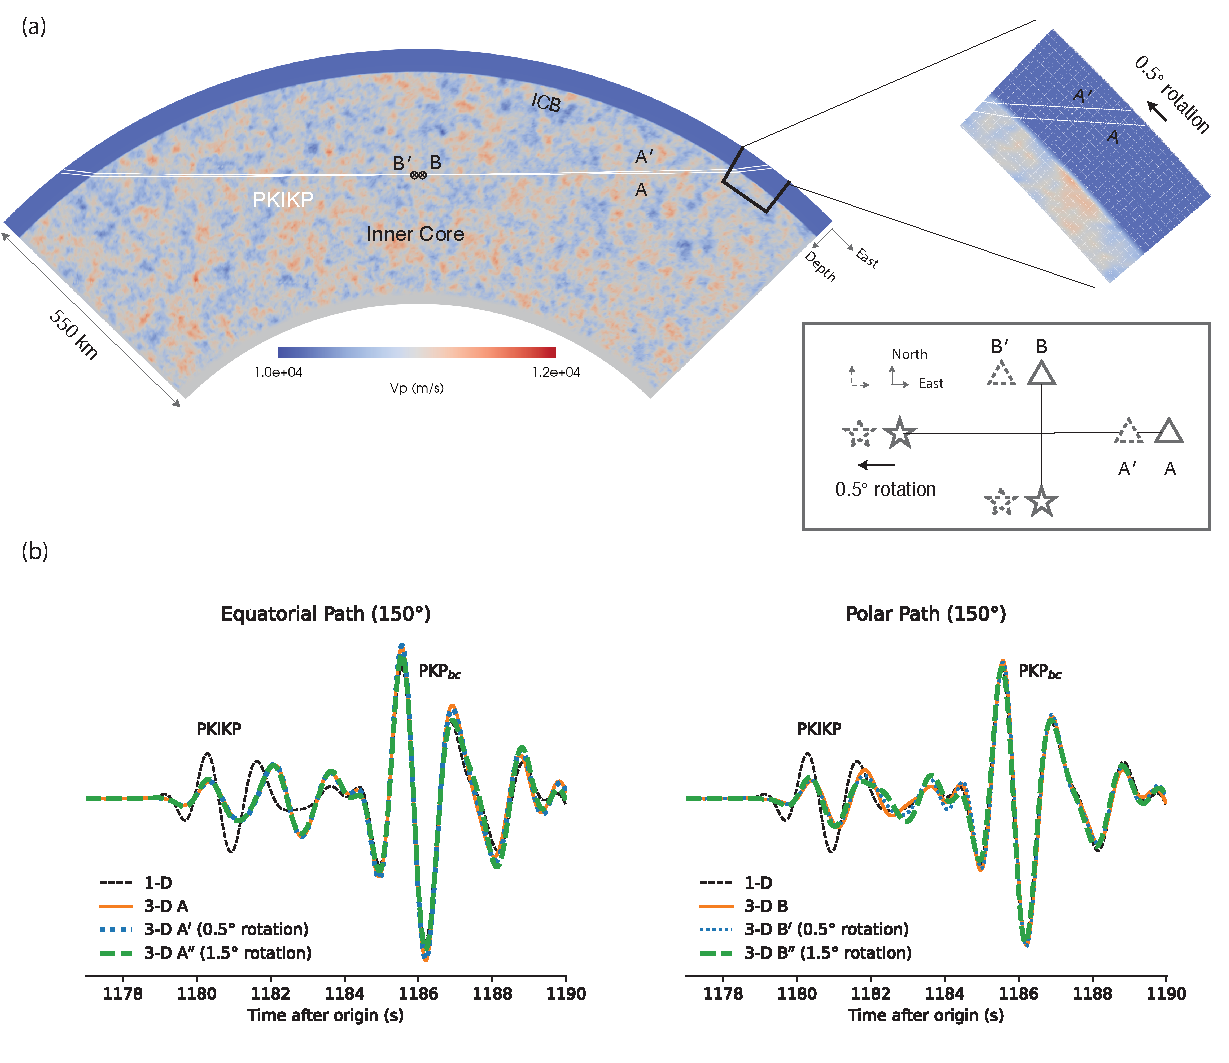
\includegraphics[width=0.86\textwidth]{PKIKP_ICrotation_ReducedSize.pdf}
  \caption{PKIKP application with rotated inner-core heterogeneity. The
  rotated model changes the 3-D structure sampled by the PKIKP path while
  preserving the same reference 1-D propagation outside the SEM box.}
  \label{fig:pkikp_rotation}
\end{figure}

\subsection{Recommended setup}

Use a box centered in the inner core along the PKIKP path. Set
\code{PHASE_SOURCE_TO_BOX} and \code{PHASE_BOX_TO_RECEIVER} to include the
internal-core phase family needed by the corner-arrival estimator, for example
\code{PKI,PK}. For initial checks, set \code{DSM1D_OR_3D = DSM1D}. For the
rotation experiment, switch to \code{DSM3D}, edit the case-local
\code{model_tomography.f90} and \code{get_model.F90} pair if needed, run
\code{./step0_prepare_*.sh --install}, and rerun the database, solver,
coupling, and assembly steps.

\subsection{Reusing DSM products}

For rotation tests, the 1-D source-to-box and box-to-receiver DSM products can
often be reused when the source, receivers, 1-D model, SEM-box geometry, and
time windows are unchanged. The reusable-product controls are:
\begin{lstlisting}
DSM_SRC_TO_BOX_DIR =
DSM_BOX_TO_RECV_DIR =
INJECTED_WAVEFIELD_PATH =
INJECTED_WAVES_METADATA =
COUPLING_DSM_BOX_TO_RECV_DIR =
\end{lstlisting}
Keep these blank for a clean end-to-end run. Set them only when you have
verified that the current case geometry and DSM model are identical to the
saved product.

\subsection{Interpreting output}

The useful diagnostic comparison is between the \code{DSM1D} result and the
\code{DSM3D} rotated-model result. The difference isolates the waveform effect
of inner-core heterogeneity and its rotation. Also compare equatorial and
polar paths, because the same rotated heterogeneity can affect them
differently.

\begin{figure}[htbp]
  \centering
  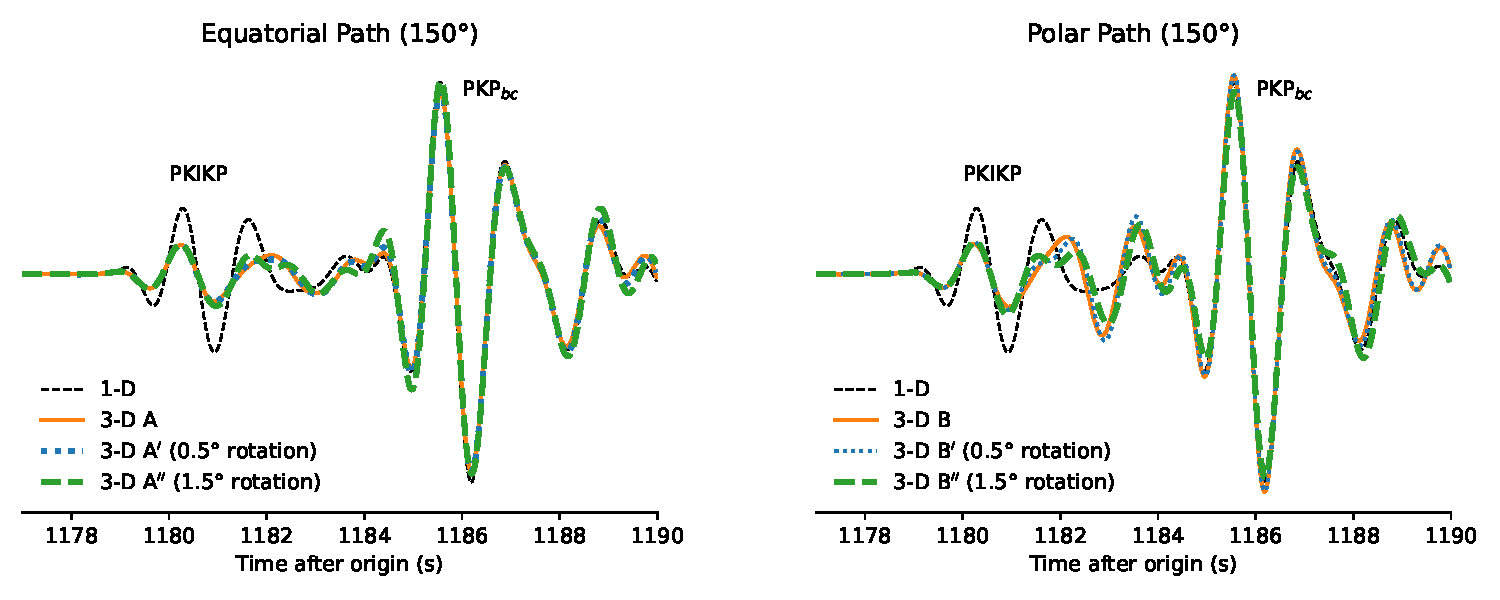
\includegraphics[width=0.86\textwidth]{PKIKP_150deg_equator_polar_comparison.pdf}
  \caption{Example comparison of equatorial and polar PKIKP paths. Use this
  type of comparison to separate path geometry from the imposed rotation of
  inner-core structure.}
  \label{fig:pkikp_equator_polar}
\end{figure}

\section{PKiKP with ICB topography}
\label{sec:pkikp_icb_topography}

This example models PKiKP reflections from inner-core boundary topography. The
example directories include:
\begin{lstlisting}
example/PKiKP_ICB_topo_demo/Explosion_demo
example/PKiKP_ICB_topo_demo/Explosion_DSM_database_existing_demo
\end{lstlisting}

\begin{figure}[htbp]
  \centering
  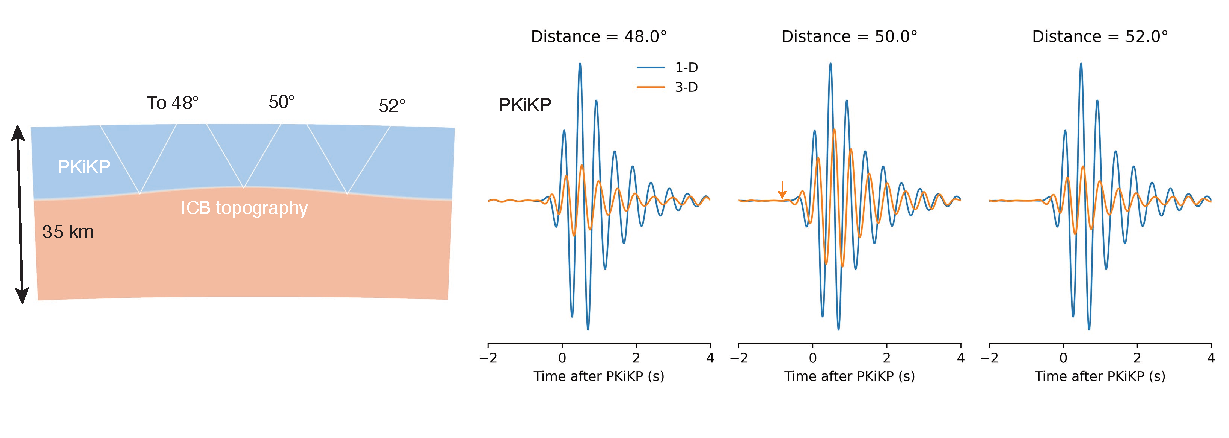
\includegraphics[width=0.86\textwidth]{PKiKP_ReducedSize.pdf}
  \caption{PKiKP application with ICB topography. The SEM box surrounds the
  reflection region, while the source-side and receiver-side propagation are
  handled by DSM in the 1-D background model.}
  \label{fig:pkikp_topography}
\end{figure}

\subsection{Topography preparation}

The PKiKP example uses an ICB topography file such as:
\begin{lstlisting}
DATA/topo_files/latlon_ICB_topo.txt
\end{lstlisting}
The parameter \code{ICB_TOPOGRAPHY_FILE} points to this file. During database
preparation, the topography is converted to the cubed-sphere interface format.

After setting \code{DSM1D_OR_3D}, run
\code{./step0_prepare_model.sh --install}. In addition to installing the two
Fortran sources and rebuilding \code{xgenerate_databases}, the \code{DSM3D}
path generates the ICB topography input before mesh preparation.

\subsection{Parameter choices}

PKiKP is small, so numerical mismatch can be visible. Use the high-resolution
coupling boundary:
\begin{lstlisting}
LOW_RESOLUTION = .false.
\end{lstlisting}
Use conservative mesh settings near the ICB and test \code{DSM1D} before
interpreting topography. The example uses a relatively high
\code{OUTER_CORE_ELEMENTS_PER_WAVELENGTH} because the coupling includes waves
that propagate through the fluid outer core and reflect near the ICB.

\subsection{Suggested run sequence}

For a clean PKiKP topography run:
\begin{lstlisting}
# 1-D consistency check
set DSM1D_OR_3D = DSM1D in DATA/Par_file_SEM_DSM
./step0_prepare_model.sh --install
./step1_specfem_mesh_database.sh
./step3_submit_specfem_mesh_gen.sh
./step4_dsm_src_to_box.sh
./step5_dsm_box_to_recv.sh
./step6_1d_dsm_synthetics.sh
./step7_extract_injected_waves.sh
./step8_specfem_solver.sh
./step9_coupling.sh
./step10_assemble_3d_sem_dsm_synthetics.sh

# 3-D ICB topography run
set DSM1D_OR_3D = DSM3D in DATA/Par_file_SEM_DSM
./step0_prepare_model.sh --install
./step1_specfem_mesh_database.sh
./step3_submit_specfem_mesh_gen.sh
./step8_specfem_solver.sh
./step9_coupling.sh
./step10_assemble_3d_sem_dsm_synthetics.sh
\end{lstlisting}
When the source, stations, 1-D model, and SEM-box geometry are unchanged, the
DSM products from the 1-D check can be reused for the 3-D topography run.

\begin{figure}[htbp]
  \centering
  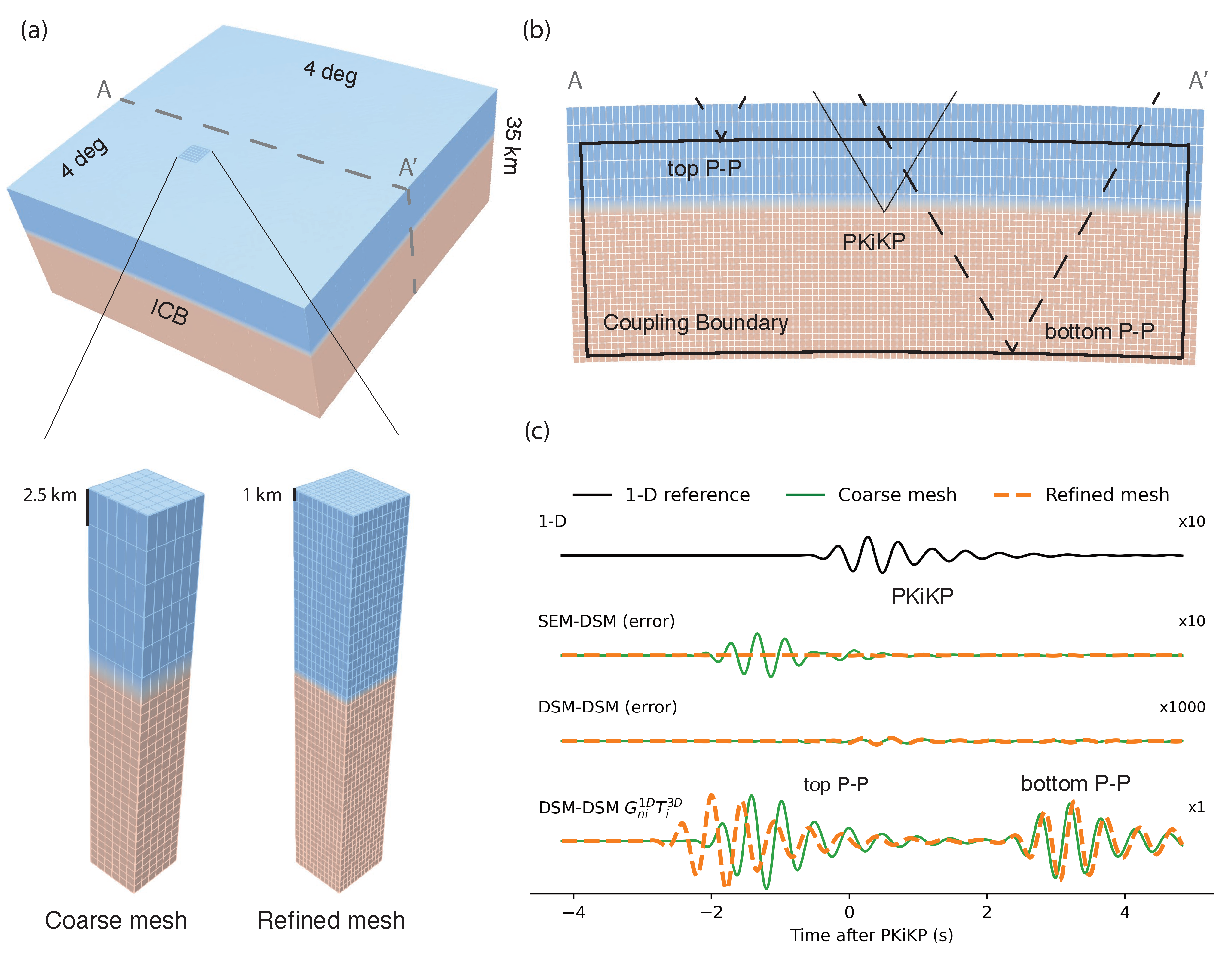
\includegraphics[width=0.86\textwidth]{PKiKP_1D_ReducedSize.pdf}
  \caption{PKiKP 1-D benchmark. This type of test is used to quantify
  SEM--DSM numerical mismatch before adding ICB topography.}
  \label{fig:pkikp_1d}
\end{figure}

\section{Output organization}

Although examples differ in model details, the final products usually appear
under:
\begin{lstlisting}
WORK/Coupling/OUTPUT_FILES/
WORK/DSM/1D_tele_syn/
OUTPUT_FILES_DSM1D_*
OUTPUT_FILES_DSM3D_*
\end{lstlisting}
Use the \code{DSM1D} and \code{DSM3D} directories as paired products: the
\code{DSM1D} run quantifies numerical error and the \code{DSM3D} run contains
the target structural signal plus the same numerical background.

\backmatter
\chapter{Troubleshooting}

\begin{longtable}{L{0.32\textwidth}L{0.58\textwidth}}
\toprule
Symptom & Likely fix \\
\midrule
\code{dsmti} not found & Build \code{src/DSM/src/DSM_Solver} or correct the
relative path in the case scripts. \\
\code{extract_Injectedwaves} not found & Build \code{src/InjectedWaves/src}
or set \code{EXTRACT_INJECTEDWAVES_BIN}. \\
\code{coupling_integral} not found & Build \code{src/Coupling/src} or set
\code{COUPLING_INTEGRAL_BIN}. \\
Injected-wave step stops because SEM depth tables are missing & Wait for
\code{xmeshfem3D} and \code{xgenerate_databases} to finish successfully. \\
\code{xgenerate_databases} is missing, stale, or built for another case & Run
\code{./step0_prepare_*.sh --install} from the intended case directory, then
rerun Step~3. \\
SPECFEM3D solver overflows & Reduce \code{SPECFEM3D_SOLVER_DT}, reduce the
injected-wave frequency band, or inspect the injected-wave cut window. \\
Large scattered waveform in \code{DSM1D} mode & Check DSM-model consistency,
mesh resolution, coupling-boundary placement, and \code{LOW_RESOLUTION}. \\
Coupling job runs out of memory & Increase \code{COUPLING_MEM_PER_CPU}, reduce
the receiver/component set, or split the coupling job. \\
Final 3-D synthetics are missing the reference phase & Run
\code{step6_1d_dsm_synthetics.sh} and then rerun
\code{step10_assemble_3d_sem_dsm_synthetics.sh}. \\
\bottomrule
\end{longtable}

\end{document}
